\documentclass[12pt,a4paper]{article}
\usepackage{ctex}
\usepackage{geometry}
\usepackage{graphicx}
\usepackage{setspace}
\usepackage{listings}
\usepackage{listingsutf8}
\usepackage{xcolor}
\usepackage{float} 
\usepackage[colorlinks=true,linkcolor=blue]{hyperref}

\geometry{left=3cm,right=3cm,top=2.5cm,bottom=2.5cm}

% 代码样式
\lstset{
    language=Java,
    inputencoding=utf8,
    basicstyle=\ttfamily\small,
    keywordstyle=\color{blue}\bfseries,
    commentstyle=\color{green!50!black},
    stringstyle=\color{orange},
    showstringspaces=false,
    numbers=left,
    numberstyle=\tiny,
    breaklines=true,
    frame=single
}

\begin{document}

% ================= 封面 =================
\begin{titlepage}
\centering

% 校徽 Logo 
\makebox[\textwidth][c]{%
  
\includegraphics[height=4cm]{fengmian.png}%
}
\vspace*{2cm}

% 学院名称
{\zihao{1}\heiti 信息科学与工程学院}\\[1cm]

% 学年学期
{\zihao{4} 2025---2026 \kaishu学年第一学期}\\[1.5cm]

% 报告标题
\makebox[\textwidth][c]{%
  
\includegraphics[height=2cm]{shiyanbaogao.png}%
}
\\[2em] % 空行
% 实验基本信息表
\zihao{4} 
\renewcommand{\arraystretch}{1.8} % 表格行距
\begin{tabular}{rl}
\heiti 课程名称: & \underline{\makebox[18em][c]{\fangsong Java 编程技术}} \\
\vspace{1cm}
\heiti 实验名称: & \underline{\makebox[18em][c]{\fangsong 第四次实验}} \\
\kaishu 专  业  班  级 & \underline{\makebox[18em][c]{\kaishu 通信一班}} \\
\kaishu 学  生  学  号 & \underline{\makebox[18em][c]{\kaishu 202300120317}} \\
\kaishu 学  生  姓  名 & \underline{\makebox[18em][c]{\kaishu 陈都阳}} \\
\kaishu 实  验  时  间 & \underline{\makebox[18em][c]{\kaishu 2025年10月16日}} \\
\end{tabular}

\vfill
\end{titlepage}

% ================= 正文 =================
\section*{【实验目的】}
\begin{enumerate}
    \item 掌握数组与字符串的基本操作,熟悉常用方法的使用。
    \item 理解类与对象的概念,掌握方法重载、this 与 super 的用法。
    \item 学习使用 Calendar、Date 类,完成万年历程序设计。
    \item 了解集合 List、Map、Set 及 Stream 流操作的基本应用。
\end{enumerate}

\section*{【实验要求】}
\begin{enumerate}
    \item 按实验内容要求完成各部分程序,代码需包含必要注释。
    \item 编译运行程序,并截图保存实验结果。
    \item 在实验报告中写明实验思路、核心代码分析及实验心得。
\end{enumerate}

\section*{【第一个实验具体内容】}
代码框在不同平台上兼容的问题,代码部分的注释翻译成英文了,原版代码请查看代码支撑材料。
\subsection*{流程图}

\begin{figure}[H]
\centering
\includegraphics[width=0.8\textwidth,height=0.8\textheight,keepaspectratio]{onea1.png}
\caption{流程图}
\end{figure}

\subsection*{源代码说明}
该程序生成指定大小的整数数组并用随机数填充,打印原始数据以便检查。实现对数组的统计分析(最大值、最小值、求和与平均值)并输出结果。使用 Arrays.sort 对数组进行排序并展示排序后的内容。点击查看\hyperref[sec:one]{One.java完整代码}。

\subsection*{实验过程与结果}

\begin{figure}[H]
\centering
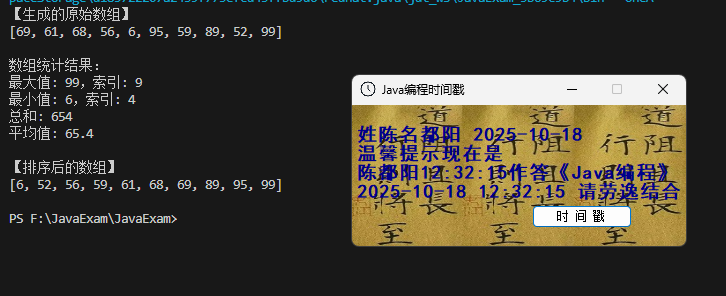
\includegraphics[width=0.8\textwidth,height=0.8\textheight,keepaspectratio]{onea.png}
\caption{运行结果}
\end{figure}

\section*{【第二个实验具体内容】}
\subsection*{流程图}

\begin{figure}[H]
\centering
% 限制图片最大高度以避免 "Dimension too large" 错误,同时保持宽度为 0.8\textwidth
\includegraphics[width=0.8\textwidth,height=0.8\textheight,keepaspectratio]{twoa1.png}
\caption{流程图}
\end{figure}

\subsection*{源代码说明}
演示数组复制与多维数组遍历的典型用法。使用 System.arraycopy 和 Arrays.copyOf 实现完整、部分及扩展复制并打印结果。展示二维与三维数组的遍历与输出以验证索引访问与格式化打印。点击查看\hyperref[sec:two]{Two.java完整代码}。

\subsection*{实验过程与结果}

\begin{figure}[H]
\centering
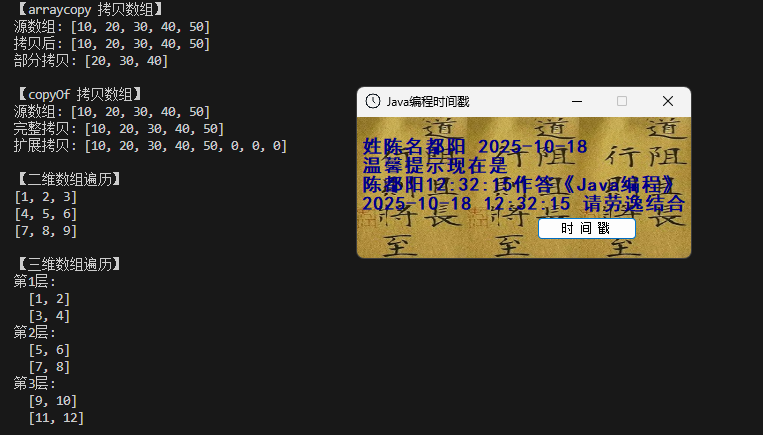
\includegraphics[width=0.8\textwidth,height=0.8\textheight,keepaspectratio]{twoa.png}
\caption{运行结果}
\end{figure}

\section*{【第三个实验具体内容】}
\subsection*{流程图}

\begin{figure}[H]
\centering
\includegraphics[width=0.8\textwidth,height=0.8\textheight,keepaspectratio]{threea1.png}
\caption{流程图}
\end{figure}

\subsection*{源代码说明}
展示字符串分析与可变字符序列的基本操作。使用 String 的常用方法(length、charAt、substring、lastIndexOf)对字符串进行提取与分析。使用 StringBuffer 演示替换、插入与追加等可变字符操作并输出中间结果。点击查看\hyperref[sec:three]{Three.java完整代码}。

\subsection*{实验过程与结果}

\begin{figure}[H]
\centering
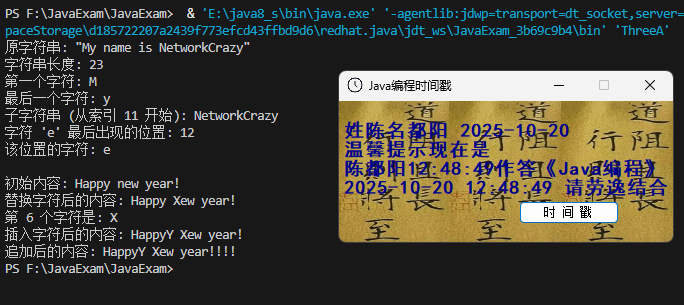
\includegraphics[width=0.8\textwidth,height=0.8\textheight,keepaspectratio]{threea.png}
\caption{运行结果}
\end{figure}

\section*{【第四个实验具体内容】}
\subsection*{流程图}

\begin{figure}[H]
\centering
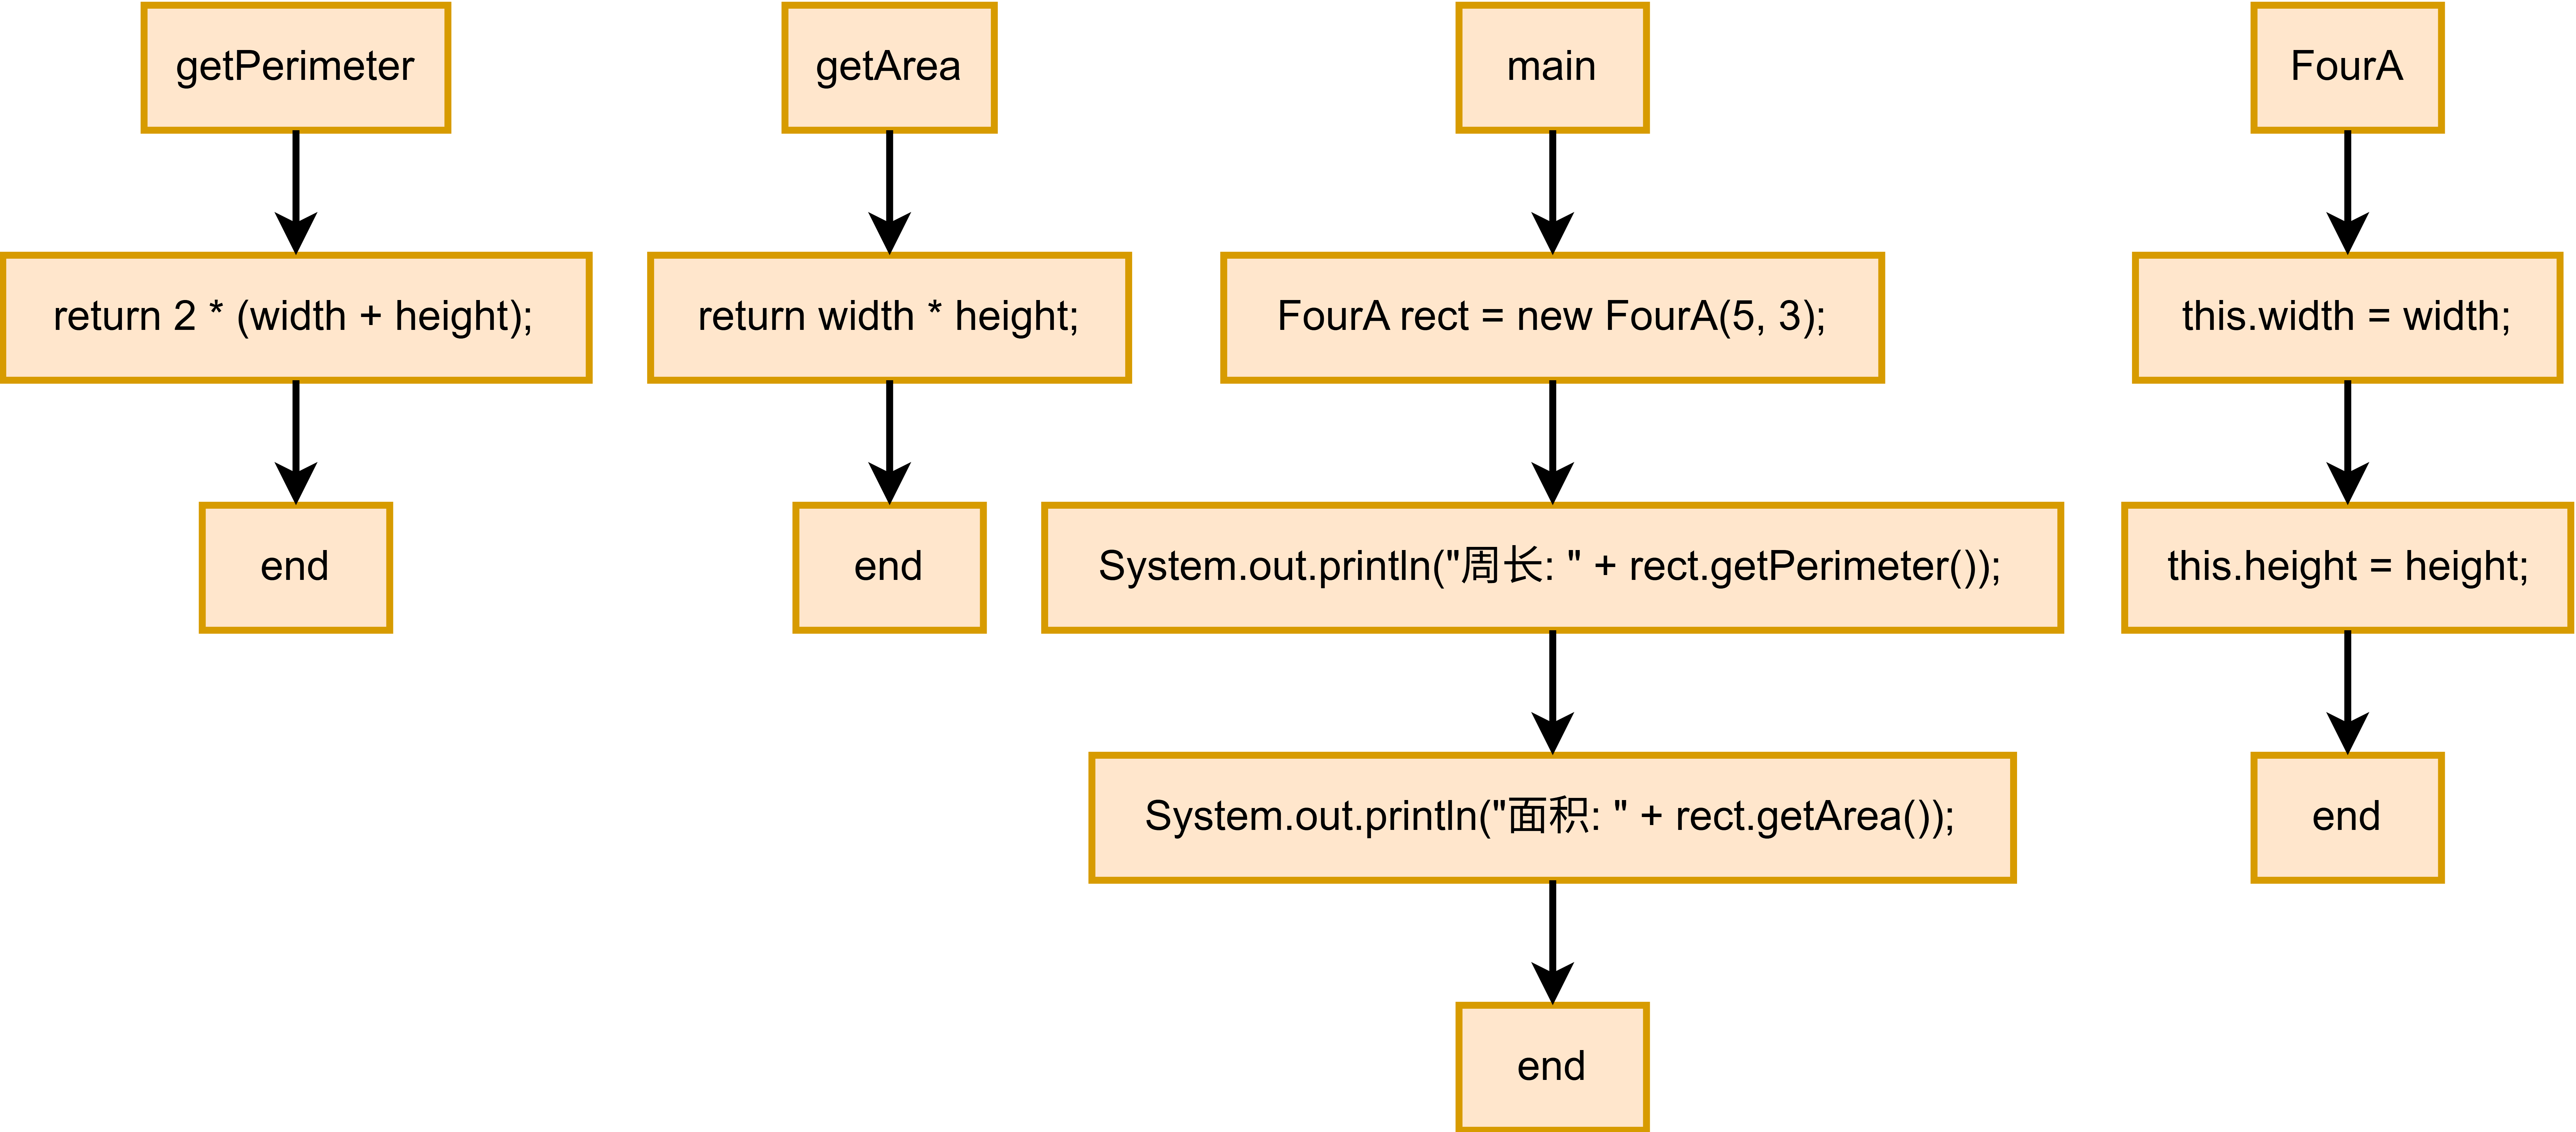
\includegraphics[width=0.8\textwidth,height=0.8\textheight,keepaspectratio]{foura1.png}
\caption{流程图}
\end{figure}

\subsection*{源代码说明}
实现了矩形类并封装宽与高的属性,通过构造器初始化。提供计算周长(getPerimeter)和面积(getArea)的方法并在 main 中实例化验证。代码侧重面向对象的封装与方法设计。点击查看\hyperref[sec:four]{Four.java完整代码}。

\subsection*{实验过程与结果}

\begin{figure}[H]
\centering
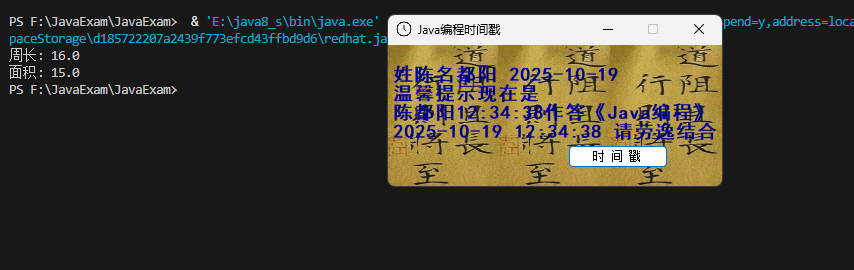
\includegraphics[width=0.8\textwidth,height=0.8\textheight,keepaspectratio]{foura.png}
\caption{运行结果}
\end{figure}

\section*{【第五个实验具体内容】}
\subsection*{流程图}

\begin{figure}[H]
\centering
\includegraphics[width=0.8\textwidth,height=0.8\textheight,keepaspectratio]{fivea1.png}
\caption{流程图}
\end{figure}

\subsection*{源代码说明}
定义抽象类 Shape 并由 Triangle、Ladder(梯形)与 Circle 实现具体计算。各子类实现周长与面积的方法,主程序通过多态遍历 Shape 数组并输出结果。代码演示抽象、继承与运行时多态的基本用法。点击查看\hyperref[sec:five]{Five.java完整代码}。

\subsection*{实验过程与结果}

\begin{figure}[H]
\centering
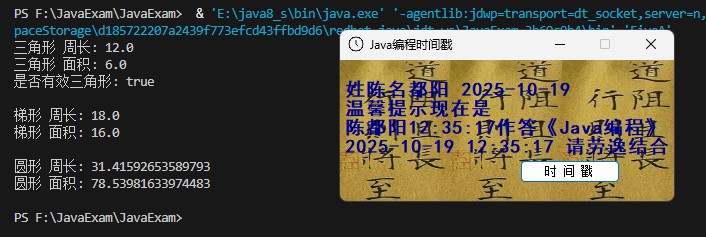
\includegraphics[width=0.8\textwidth,height=0.8\textheight,keepaspectratio]{fivea.png}
\caption{运行结果}
\end{figure}

\section*{【第六个实验具体内容】}
\subsection*{流程图}

\begin{figure}[H]
\centering
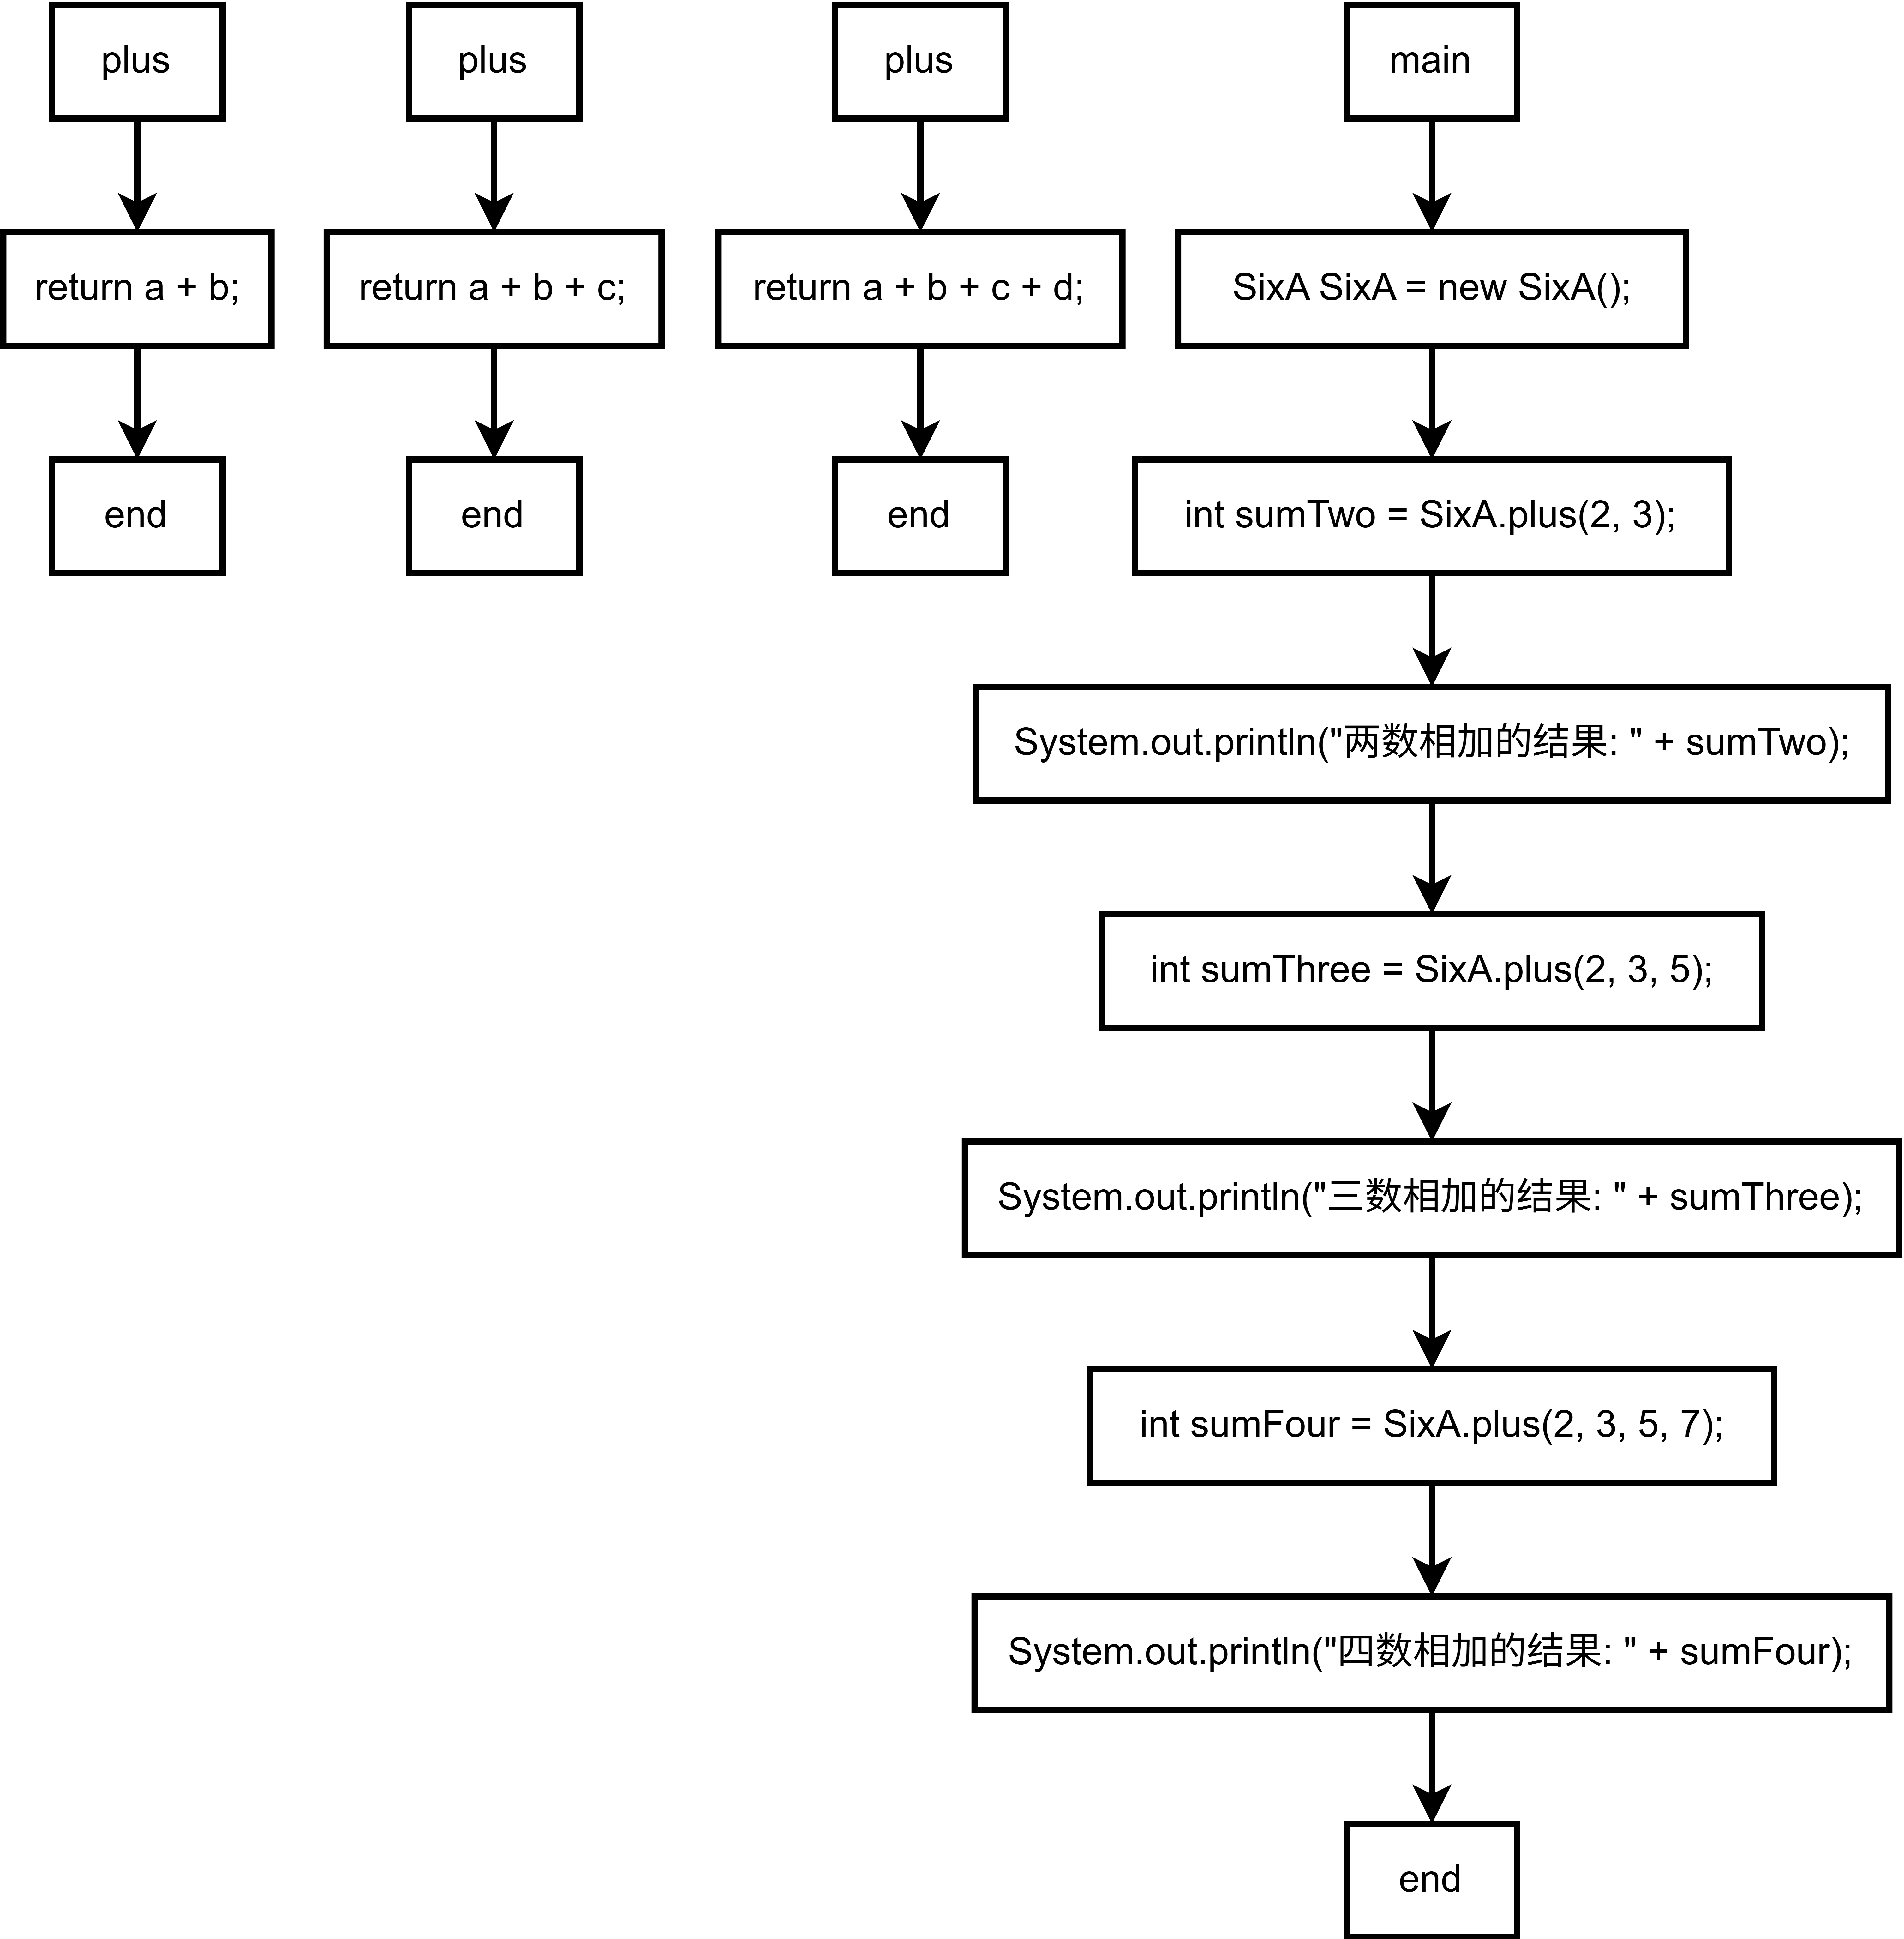
\includegraphics[width=0.8\textwidth,height=0.8\textheight,keepaspectratio]{sixa1.png}
\caption{流程图}
\end{figure}

\subsection*{源代码说明}
通过方法重载实现加法的多个版本(支持 2、3、4 个参数),展示参数个数不同的重载规则。主程序调用不同重载方法并打印结果以验证分派行为。代码简洁,便于学习重载机制。点击查看\hyperref[sec:six]{Six.java完整代码}。

\subsection*{实验过程与结果}

\begin{figure}[H]
\centering
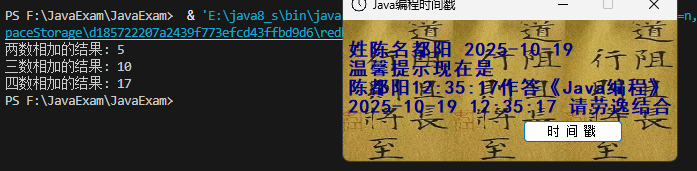
\includegraphics[width=0.8\textwidth,height=0.8\textheight,keepaspectratio]{sixa.png}
\caption{运行结果}
\end{figure}

\section*{【第七个实验具体内容】}
\subsection*{流程图}

\begin{figure}[H]
\centering
\includegraphics[width=0.8\textwidth,height=0.8\textheight,keepaspectratio]{sevena1.png}
\caption{流程图}
\end{figure}

\subsection*{源代码说明}
演示继承、super 与 this 的常见用法。定义基类 Person 与子类 ZhangSan,子类覆盖方法并在示例中调用 super.printPerson() 与 this.printPerson()。通过输出比较 super/this/局部变量的字段值与调用顺序。点击查看\hyperref[sec:seven]{Seven.java完整代码}。


\subsection*{实验过程与结果}

\begin{figure}[H]
\centering
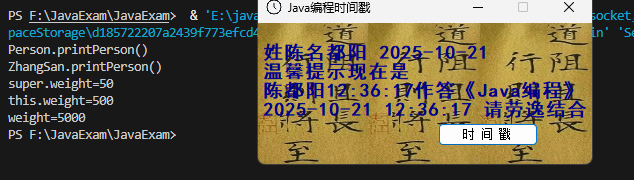
\includegraphics[width=0.8\textwidth,height=0.8\textheight,keepaspectratio]{sevena.png}
\caption{运行结果}
\end{figure}

\section*{【第八个实验具体内容】}
\subsection*{流程图}

\begin{figure}[H]
\centering
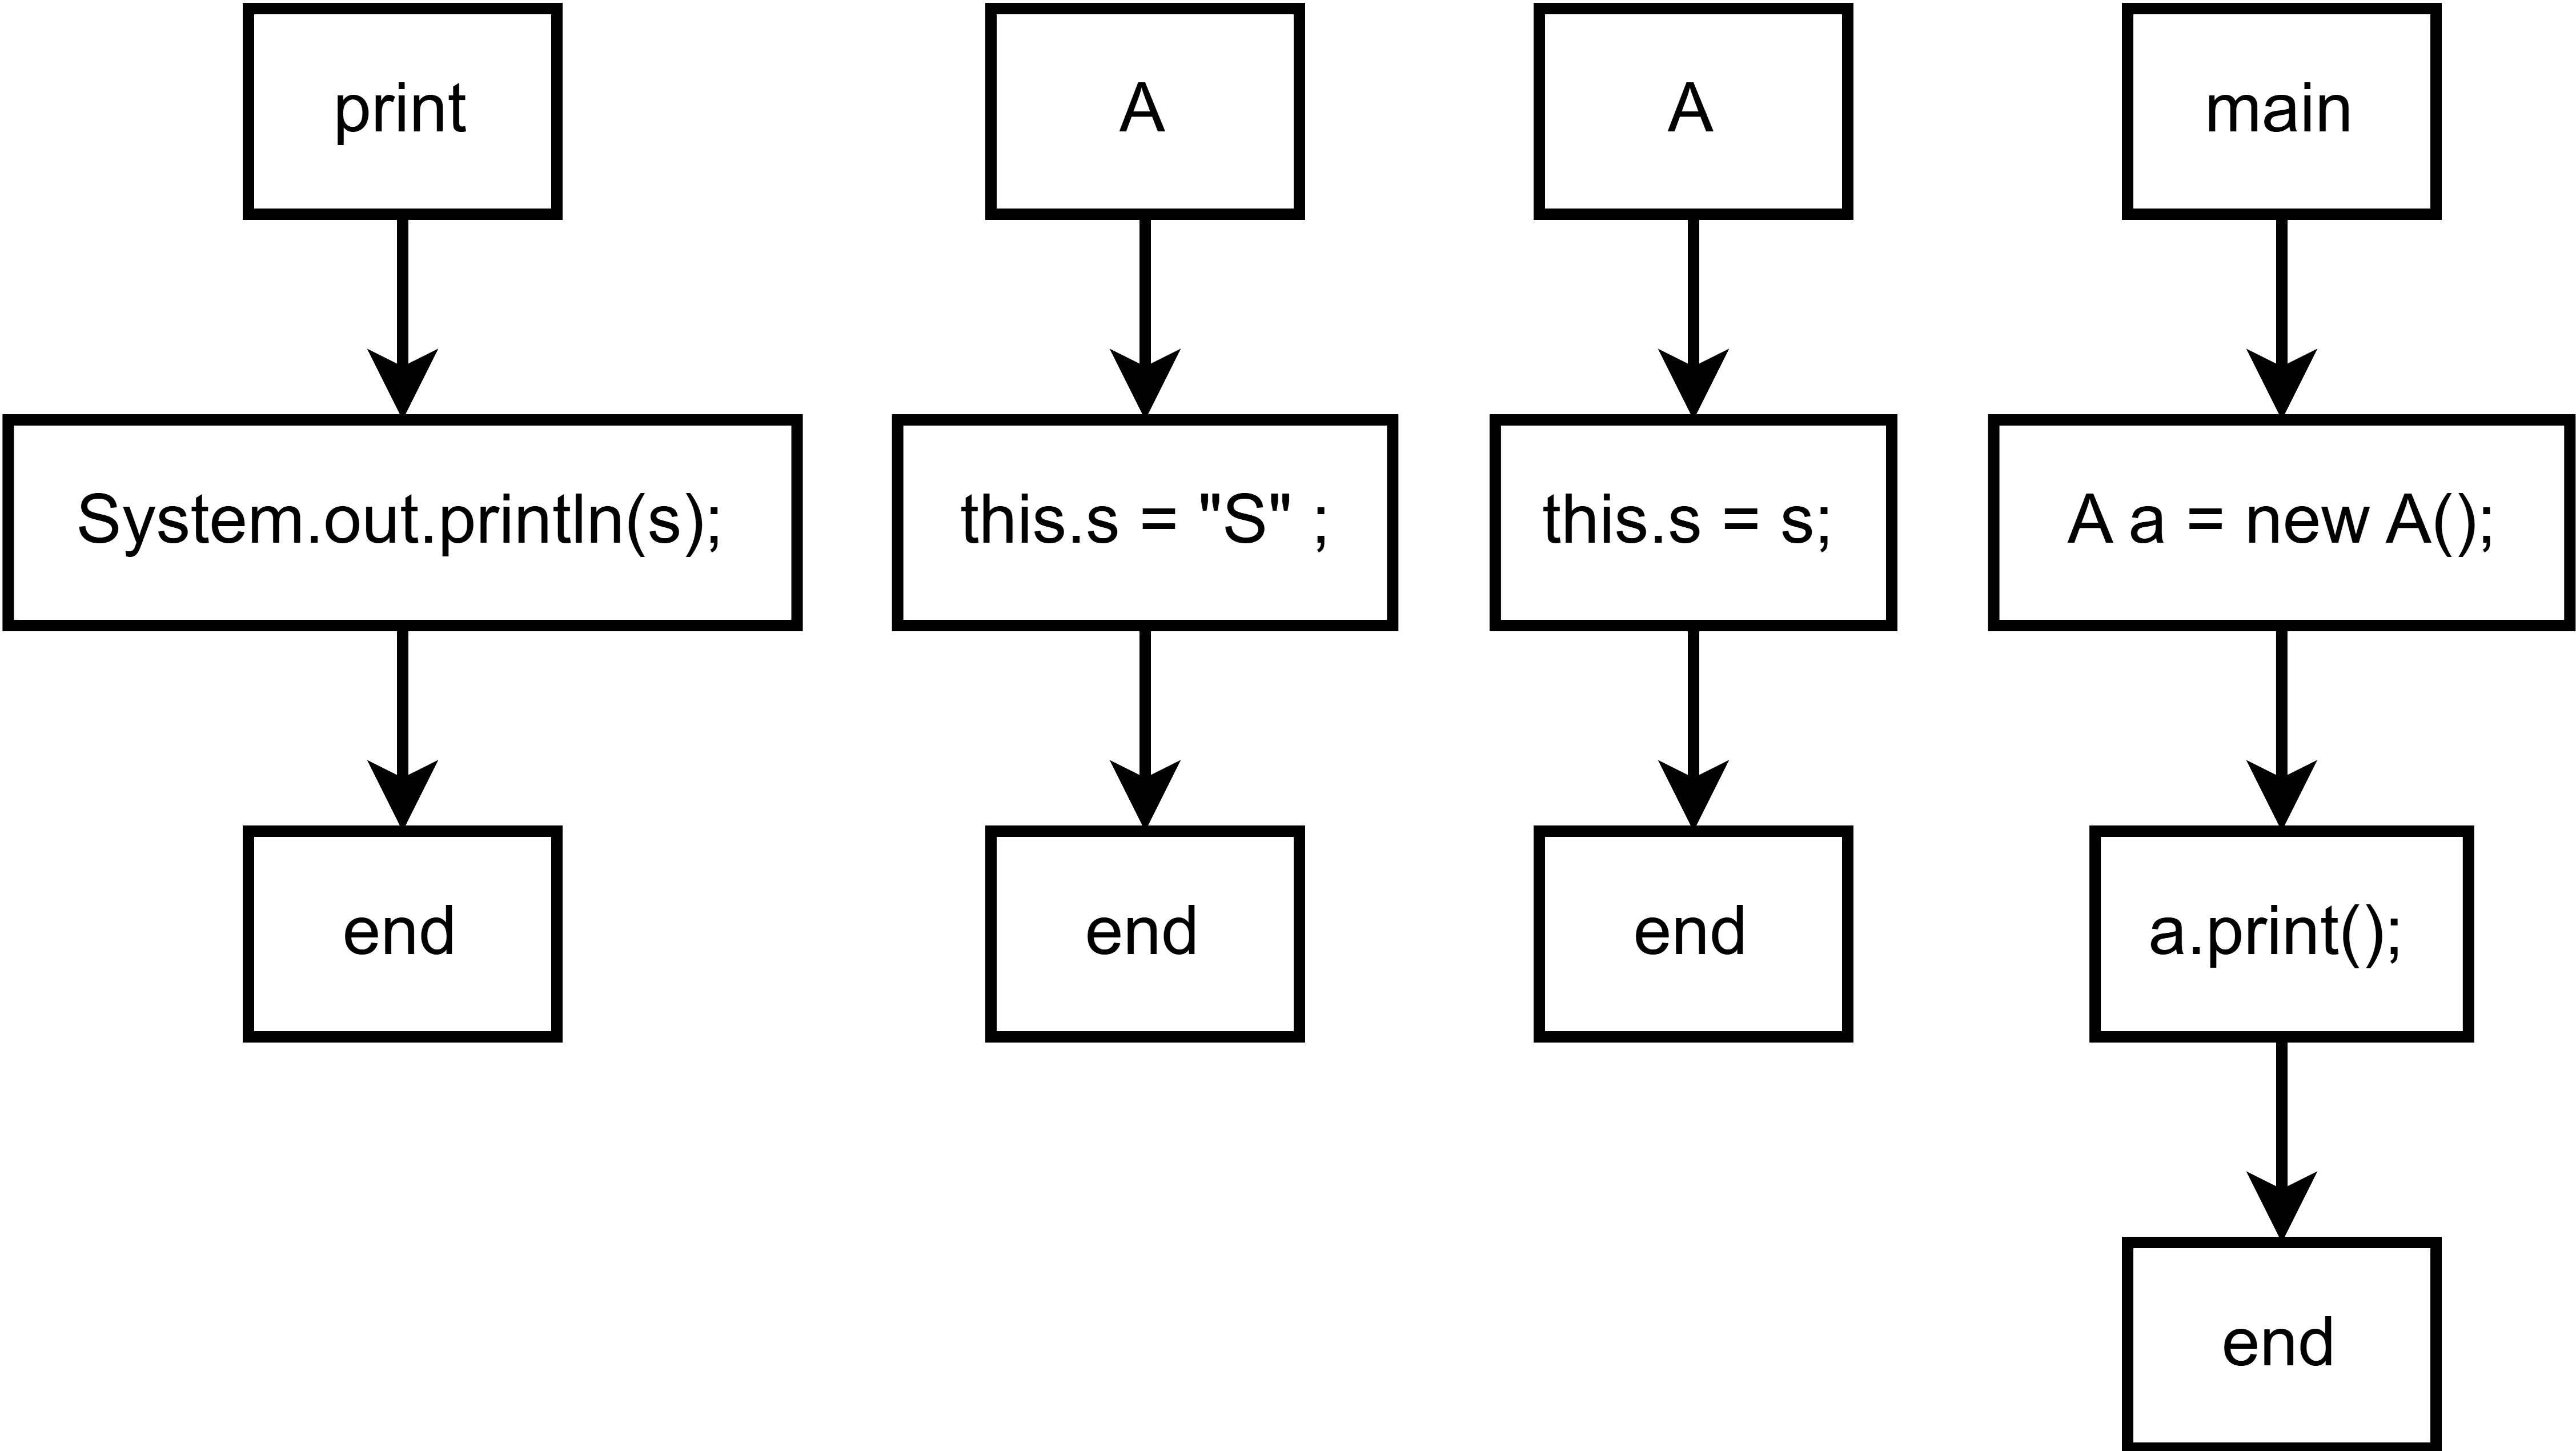
\includegraphics[width=0.8\textwidth,height=0.8\textheight,keepaspectratio]{eighta1.png}
\caption{流程图}
\end{figure}

\subsection*{源代码说明}
本实验的源代码 (Eight.java) 说明了构造器重载与默认构造器:
提供无参构造器与带参构造器,并在 print 方法中输出实例字段的值。
在 main 中创建 A 的实例并调用 print,展示构造器初始化行为。点击查看\hyperref[sec:eight]{Eight.java完整代码}。

\subsection*{实验过程与结果}

\begin{figure}[H]
\centering
% 限制图片最大高度以避免 "Dimension too large" 错误,同时保持宽度为 0.8\textwidth
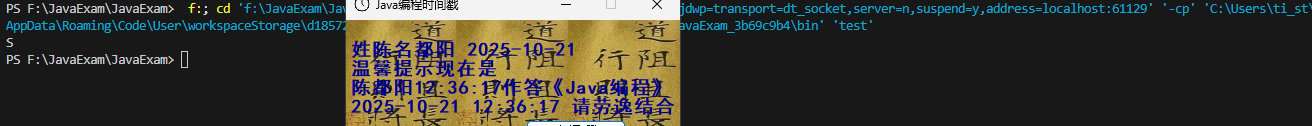
\includegraphics[width=0.8\textwidth,height=0.8\textheight,keepaspectratio]{eighta.png}
\caption{运行结果}
\end{figure}

\section*{【第九个实验具体内容】}
\subsection*{流程图}

\begin{figure}[H]
\centering
\includegraphics[width=0.8\textwidth,height=0.8\textheight,keepaspectratio]{ninea1.png}
\caption{流程图}
\end{figure}

\subsection*{源代码说明}
本实验的源代码 (Nine.java) 实现了一个基于 Swing 的简易万年历与日程管理器:
使用 YearMonth 与 LocalDate 处理年月日,显示指定月份的日历格子(refreshCalendar)。
提供上一月/下一月导航、按日期跳转输入框,以及为单日添加与查看日程的对话框(showScheduleDialog)。
使用 HashMap 将 LocalDate 映射到日程列表,实现简单的本地内存日程存储与交互。点击查看\hyperref[sec:nine]{Nine.java完整代码}。    

\subsection*{实验过程与结果}

\begin{figure}[H]
\centering
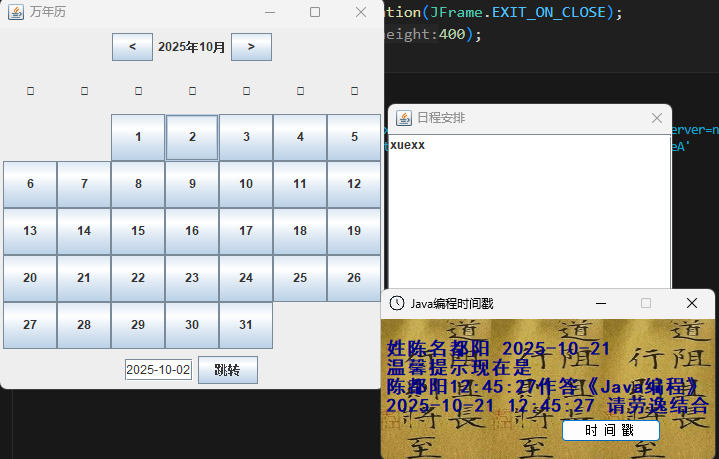
\includegraphics[width=0.8\textwidth,height=0.8\textheight,keepaspectratio]{ninea.png}
\caption{运行结果}
\end{figure}


\section*{【实验心得】}
    本次实验主要花费时间在第九个实验上了,其他实验都还比较简单,主要是考察对基本算法的理解与实现。\\

    第九个实验是一个比较完整的项目,实现了一个简易的万年历与日程管理器。通过这个实验,我加深了对 Java Swing GUI 编程的理解,学会了如何使用布局管理器、事件监听器等组件来构建交互界面。同时,利用 Java 8 的日期时间 API(YearMonth、LocalDate)处理日期相关逻辑,使得代码更加简洁易读。\\

    但是在打包成exe二进制文件时遇到了一些问题,主要是依赖打包不上,在我的电脑上可以运行,在一些缺少依赖的电脑上就无法运行。而且由于使用的Java版本为Java8,用不了jpackage工具,只能自己手动打包。在把jar包转exe时使用了exe4j工具。\\

    远不如C\#打包方便,之前一套从源码到混淆再到打包成安装包的流程在Java套用时好多环节找不到对应的替换工具\\

    由于本次实验报告体量较大,前期制作粗糙,但由于突然延长时间了,所以我拿C\#制作了一个简单的万年历程序,代码量较少,功能也比较简单,但是界面美观,打包方便。\\

    c\#程序完美的解决了排版布局等功能,背景采用了动态背景,日程管理界面得到更好的优化,可以使用储存日程,且可以直接加入电脑计划任务,实现开机自启提醒功能。\\
    
    
\newpage
\begin{center}
    {\zihao{1}\heiti 附录}
\end{center}
{\zihao{2}【代码附录】}\\

\section*{One.java源代码}\label{sec:one}
\begin{lstlisting}
// One.java
import java.util.*;
public class OneA {

    public static void main(String[] args) {
        IntArray arr = new IntArray(10);
        arr.generateRandom(100);  
        arr.print("Generated Original Array");

        arr.analyze();
        arr.sort(); 
        arr.print("Sorted Array");
    }
}

class IntArray {
    private int[] data;

    public IntArray(int size) {
        data = new int[size];
    }

    // Generate a random array
    public void generateRandom(int bound) {
        Random rand = new Random();
        for (int i = 0; i < data.length; i++) {
            data[i] = rand.nextInt(bound);
        }
    }

    // Print the array
    public void print(String title) {
        System.out.println(title);
        System.out.println(Arrays.toString(data) + "\n");
    }

    // Calculate max, min, sum, average, etc.
    public void analyze() {
        int max = data[0], min = data[0];
        int sum = 0, maxIndex = 0, minIndex = 0;

        for (int i = 0; i < data.length; i++) {
            if (data[i] > max) {
                max = data[i];
                maxIndex = i;
            }
            if (data[i] < min) {
                min = data[i];
                minIndex = i;
            }
            sum += data[i];
        }

        System.out.println("Array Analysis Results:");
        System.out.println("Maximum Value: " + max + ", Index: " + maxIndex);
        System.out.println("Minimum Value: " + min + ", Index: " + minIndex);
        System.out.println("Sum: " + sum);
        System.out.println("Average: " + (double) sum / data.length + "\n");
    }

    // Sort the array
    public void sort() {
        Arrays.sort(data);
    }
}
\end{lstlisting}

\section*{Two.java源代码}\label{sec:two}
\begin{lstlisting}
// TwoA.java
import java.util.*;
public class TwoA {
    public static void main(String[] args) {
        ArrayDemo demo = new ArrayDemo(); 
        demo.showArrayCopy();             
        demo.showCopyOf();              
        demo.show2DArray();             
        demo.show3DArray();              
    }
}

class ArrayDemo {

    /** Copy using System.arraycopy */
    public void showArrayCopy() {
        System.out.println("arraycopy Copy Array\");

        int[] src = {10, 20, 30, 40, 50};
        int[] dst = new int[src.length];
        System.arraycopy(src, 0, dst, 0, src.length);
        print("Source Array", src);
        print("Copied Array", dst);

        int[] part = new int[3];
        System.arraycopy(src, 1, part, 0, 3);
        print("Partial Copy", part);
        System.out.println();
    }

    /** Copy using Arrays.copyOf */
    public void showCopyOf() {
        System.out.println("copyOf Copy Array");

        int[] src = {10, 20, 30, 40, 50};
        print("Source Array", src);

        int[] copy = Arrays.copyOf(src, src.length);
        print("Full Copy", copy);

        int[] extend = Arrays.copyOf(src, 8);
        print("Extended Copy", extend);
        System.out.println();
    }

    /** foreach loop for 2D array */
    public void show2DArray() {
        System.out.println("2D Array Traversal");

        int[][] arr2D = {
            {1, 2, 3},
            {4, 5, 6},
            {7, 8, 9}
        };

        for (int[] row : arr2D)
            System.out.println(Arrays.toString(row));
        System.out.println();
    }

    /** foreach loop for 3D array */
    public void show3DArray() {
        System.out.println("3D Array Traversal");

        int[][][] arr3D = {
            {{1, 2}, {3, 4}},
            {{5, 6}, {7, 8}},
            {{9, 10}, {11, 12}}
        };

        for (int i = 0; i < arr3D.length; i++) {
            System.out.println("Layer " + (i + 1) + ":");
            for (int[] row : arr3D[i])
                System.out.println("  " + Arrays.toString(row));
        }
        System.out.println();
    }

    /** Print array */
    private void print(String title, int[] arr) {
        System.out.println(title + ": " + Arrays.toString(arr));
    }
}

\end{lstlisting}

\section*{Three.java源代码}\label{sec:three}
\begin{lstlisting}
// Three.java
public class ThreeA {

    public static void main(String[] args) {
        StringAnalyzer stringAnalyzer = new StringAnalyzer("My name is NetworkCrazy");
        stringAnalyzer.printBasicInfo();
        StringBufferExample stringBufferExample = new StringBufferExample("Happy new year!");
        stringBufferExample.performBufferOperations();
    }
}

class StringAnalyzer {
    private String name;

    public StringAnalyzer(String name) {
        this.name = name;
    }

    /** Print basic information about the string */
    public void printBasicInfo() {
        System.out.println("Original string: \"" + name + "\"");
        System.out.println("String length: " + name.length());
        System.out.println("First character: " + name.charAt(0));
        System.out.println("Last character: " + name.charAt(name.length() 1));
        System.out.println("Substring (starting from index 11): " + name.substring(11));
        int lastIndex = name.lastIndexOf('e');
        System.out.println("Last occurrence of character 'e': " + lastIndex);
        System.out.println("Character at that position: " + name.charAt(lastIndex));
        System.out.println();
    }
}

class StringBufferExample {
    private StringBuffer buffer;

    public StringBufferExample(String content) {
        this.buffer = new StringBuffer(content);
    }

    /** Perform StringBuffer operations */
    public void performBufferOperations() {
        System.out.println("Initial content: " + buffer.toString());
        buffer.setCharAt(6, 'X');
        System.out.println("After replacing a character: " + buffer.toString());
        char charAtPos = buffer.charAt(6);
        System.out.println("The 6th character is: " + charAtPos);
        buffer.insert(5, 'Y');
        System.out.println("After inserting a character: " + buffer.toString());
        buffer.append("!!!");
        System.out.println("After appending: " + buffer.toString());
    }
}
\end{lstlisting}

\section*{Four.java源代码}\label{sec:four}
\begin{lstlisting}
// Four.java
public class FourA {
    // Two private attributes
    private double width;
    private double height;
    
    // Constructor, taking width and height as parameters
    public FourA(double width, double height) {
        this.width = width;
        this.height = height;
    }
    
    // Calculate and return the perimeter of the rectangle
    public double getPerimeter() {
        return 2 * (width + height);
    }
    
    // Calculate and return the area of the rectangle
    public double getArea() {
        return width * height;
    }
    
    // main method for testing
    public static void main(String[] args) {
        // Create a rectangle with width = 5 and height = 3
        FourA rect = new FourA(5, 3);
        
        // Calculate and print the perimeter
        System.out.println("Perimeter: " + rect.getPerimeter());  // Output: Perimeter: 16.0
        
        // Calculate and print the area
        System.out.println("Area: " + rect.getArea());            // Output: Area: 15.0
    }
}

\end{lstlisting}


\section*{Five.java源代码}\label{sec:five}
\begin{lstlisting}
// Five.java
// Abstract class Shape
abstract class Shape {
    protected String name;
    
    public Shape(String name) {
        this.name = name;
    }
    
    // Abstract method: calculate perimeter
    public abstract double getPerimeter();
    
    // Abstract method: calculate area
    public abstract double getArea();
    
    // Common method: print information
    public void printInfo() {
        System.out.println(name + " Perimeter: " + getPerimeter());
        System.out.println(name + " Area: " + getArea());
    }
}

// Triangle class
class Triangle extends Shape { 
    private double side1;
    private double side2;
    private double side3;
    private boolean isValid;

    public Triangle(double s1, double s2, double s3) { 
        super("Triangle");
        this.side1 = s1;
        this.side2 = s2;
        this.side3 = s3;
        this.isValid = checkValidity();
    }

    private boolean checkValidity() {
        return (side1 + side2 > side3) && 
               (side1 + side3 > side2) && 
               (side2 + side3 > side1);
    }

    @Override
    public double getPerimeter() {
        return isValid ? side1 + side2 + side3 : 0;
    }

    @Override
    public double getArea() {
        if (!isValid) return 0;
        double s = getPerimeter() / 2;
        return Math.sqrt(s * (s side1) * (s side2) * (s side3));
    }

    public boolean isValid() {
        return isValid;
    }

    public void setSides(double s1, double s2, double s3) {
        this.side1 = s1;
        this.side2 = s2;
        this.side3 = s3;
        this.isValid = checkValidity();
    }
}

// Trapezoid class
class Ladder extends Shape {
    private double upperBase;
    private double lowerBase;
    private double leftBase;
    private double rightBase;
    private double height;

    public Ladder(double upper, double lower, double left, double right, double h) {
        super("Trapezoid");
        this.upperBase = upper;
        this.lowerBase = lower;
        this.height = h;
        this.leftBase = left;
        this.rightBase = right;
    }

    @Override
    public double getPerimeter() {
        return upperBase + lowerBase + leftBase + rightBase;
    }

    @Override
    public double getArea() {
        return (upperBase + lowerBase) * height / 2;
    }
}

// Circle class
class Circle extends Shape {
    private double radius;

    public Circle(double r) {
        super("Circle");
        this.radius = r;
    }

    @Override
    public double getPerimeter() {
        return 2 * Math.PI * radius;
    }

    @Override
    public double getArea() {
        return Math.PI * radius * radius;
    }
}

public class FiveA {
    public static void main(String[] args) {
        // Use polymorphism to handle different shapes
        Shape[] shapes = {
            new Triangle(3, 4, 5), 
            new Ladder(3, 5, 5, 5, 4),
            new Circle(5)
        };

        // Process all shapes uniformly
        for (Shape shape : shapes) {
            shape.printInfo();
            if (shape instanceof Triangle) { 
                System.out.println("Is valid triangle: " + ((Triangle)shape).isValid()); 
            }
            System.out.println();
        }
    }
}

\end{lstlisting}

\section*{Six.java源代码}\label{sec:six}
\begin{lstlisting}
// Six.java
public class SixA {

    // Add two numbers
    public int plus(int a, int b) {
        return a + b;
    }

    // Add three numbers
    public int plus(int a, int b, int c) {
        return a + b + c;
    }

    // Add four numbers
    public int plus(int a, int b, int c, int d) {
        return a + b + c + d;
    }

    public static void main(String[] args) {
        SixA sixA = new SixA();

        // Test addition of two numbers
        int sumTwo = sixA.plus(2, 3);
        System.out.println("Result of adding two numbers: " + sumTwo);

        // Test addition of three numbers
        int sumThree = sixA.plus(2, 3, 5);
        System.out.println("Result of adding three numbers: " + sumThree);

        // Test addition of four numbers
        int sumFour = sixA.plus(2, 3, 5, 7);
        System.out.println("Result of adding four numbers: " + sumFour);
    }
}

\end{lstlisting}

\section*{Seven.java源代码}\label{sec:seven}
\begin{lstlisting}
// Seven.java
// Create the Person class
class Person {
    int weight;

    // Constructor for the Person class
    Person() {
        weight = 50;
    }

    void printPerson() {
        System.out.println("Person.printPerson()");
    }
}

// Create the subclass ZhangSan that extends Person
class ZhangSan extends Person {
    int weight;

    // Constructor for the ZhangSan class
    ZhangSan() {
        // Call the constructor of the Person class
        super();
        weight = 500;
    }

    // Override the printPerson() method from Person
    void printPerson() {
        System.out.println("ZhangSan.printPerson()");
    }

    // Demonstrate the use of super and this
    void superThisUseDemo() {
        int weight;
        weight = 5000;
        // Call the printPerson() method from the Person class
        super.printPerson();
        // Call the printPerson() method from the ZhangSan class
        printPerson();
        // Show the weight value from the Person class
        System.out.println("super.weight = " + super.weight);
        // Show the weight value from the ZhangSan class
        System.out.println("this.weight = " + this.weight);
        // Show the local variable weight
        System.out.println("weight = " + weight);
    }
}

public class SevenA {
    public static void main(String[] args) {
        ZhangSan zhangsan = new ZhangSan();
        zhangsan.superThisUseDemo();
    }
}

\end{lstlisting}

\section*{Eight.java源代码}\label{sec:eight}
\begin{lstlisting}
// Eight.java
class A {
    String s;
    A(){
        this.s = "S";
    }

    // Parameterized constructor
    A(String s) {
        this.s = s;
    }

    public void print() {
        System.out.println(s);
    }
}

class Test {
    public static void main(String[] args) {
        A a = new A();
        a.print();
    }
}

\end{lstlisting}

\section*{Nine.java源代码}\label{sec:nine}
\begin{lstlisting}
// Nine.java
import javax.swing.*;
import java.awt.*;
import java.awt.event.ActionEvent;
import java.awt.event.ActionListener;
import java.time.LocalDate;
import java.time.YearMonth;
import java.time.format.DateTimeFormatter;
import java.time.format.DateTimeParseException;
import java.time.DayOfWeek;
import java.util.ArrayList;
import java.util.HashMap;
import java.util.List;
import java.util.Map;

public class NineA {
    private JFrame frame;
    private JButton prevMonthButton;
    private JButton nextMonthButton;
    private JLabel monthYearLabel;
    private JPanel calendarPanel;
    private YearMonth currentYearMonth;
    private Map<LocalDate, List<String>> scheduleMap; // store schedules
    private JTextField dateInputField;
    private JButton goToDateButton;

    public NineA() {
        currentYearMonth = YearMonth.now();
        scheduleMap = new HashMap<>();

        // Initialize main frame
        frame = new JFrame("Calendar");
        frame.setDefaultCloseOperation(JFrame.EXIT_ON_CLOSE);
        frame.setSize(400, 400);

        // Main content panel
        JPanel contentPanel = new JPanel(new BorderLayout());
        frame.add(contentPanel);

        // Month navigation buttons
        prevMonthButton = new JButton("<");
        nextMonthButton = new JButton(">");
        monthYearLabel = new JLabel(currentYearMonth.format(DateTimeFormatter.ofPattern("yyyy-MM")));
        JPanel monthControlPanel = new JPanel();
        monthControlPanel.add(prevMonthButton);
        monthControlPanel.add(monthYearLabel);
        monthControlPanel.add(nextMonthButton);
        contentPanel.add(monthControlPanel, BorderLayout.NORTH);

        // Date jump panel
        dateInputField = new JTextField("yyyy-MM-dd");
        goToDateButton = new JButton("Go");
        JPanel dateControlPanel = new JPanel();
        dateControlPanel.add(dateInputField);
        dateControlPanel.add(goToDateButton);
        contentPanel.add(dateControlPanel, BorderLayout.SOUTH);

        // Calendar panel
        calendarPanel = new JPanel(new GridLayout(0, 7));
        contentPanel.add(calendarPanel, BorderLayout.CENTER);

        // Event listeners for month navigation
        prevMonthButton.addActionListener(new ActionListener() {
            @Override
            public void actionPerformed(ActionEvent e) {
                currentYearMonth = currentYearMonth.minusMonths(1);
                monthYearLabel.setText(currentYearMonth.format(DateTimeFormatter.ofPattern("yyyy-MM")));
                refreshCalendar();
            }
        });

        nextMonthButton.addActionListener(new ActionListener() {
            @Override
            public void actionPerformed(ActionEvent e) {
                currentYearMonth = currentYearMonth.plusMonths(1);
                monthYearLabel.setText(currentYearMonth.format(DateTimeFormatter.ofPattern("yyyy-MM")));
                refreshCalendar();
            }
        });

        // Jump to date event
        goToDateButton.addActionListener(new ActionListener() {
            @Override
            public void actionPerformed(ActionEvent e) {
                String dateText = dateInputField.getText();
                try {
                    LocalDate date = LocalDate.parse(dateText, DateTimeFormatter.ofPattern("yyyy-MM-dd"));
                    currentYearMonth = YearMonth.from(date);
                    monthYearLabel.setText(currentYearMonth.format(DateTimeFormatter.ofPattern("yyyy-MM")));
                    refreshCalendar();
                } catch (DateTimeParseException ex) {
                    JOptionPane.showMessageDialog(frame, "Invalid date format. Use yyyy-MM-dd.", "Error", JOptionPane.ERROR_MESSAGE);
                }
            }
        });

        // Show calendar
        refreshCalendar();
        frame.setVisible(true);
    }

    private void refreshCalendar() {
        calendarPanel.removeAll();
        DayOfWeek firstDayOfMonth = currentYearMonth.atDay(1).getDayOfWeek();
        int daysInMonth = currentYearMonth.lengthOfMonth();

        // Weekday labels
        String[] daysOfWeek = {"Sun", "Mon", "Tue", "Wed", "Thu", "Fri", "Sat"};
        for (String day : daysOfWeek) {
            JLabel label = new JLabel(day, SwingConstants.CENTER);
            label.setFont(new Font("Arial", Font.BOLD, 12));
            calendarPanel.add(label);
        }

        // Empty cells before the first day
        for (int i = DayOfWeek.MONDAY.getValue(); i < firstDayOfMonth.getValue(); i++) {
            calendarPanel.add(new JLabel());
        }

        // Date buttons
        for (int day = 1; day <= daysInMonth; day++) {
            JButton dayButton = new JButton(String.valueOf(day));
            dayButton.addActionListener(new ActionListener() {
                @Override
                public void actionPerformed(ActionEvent e) {
                    LocalDate date = currentYearMonth.atDay(Integer.parseInt(((JButton) e.getSource()).getText()));
                    // Open schedule dialog
                    showScheduleDialog(date);
                }
            });
            calendarPanel.add(dayButton);
        }

        calendarPanel.revalidate();
        calendarPanel.repaint();
    }

    private void showScheduleDialog(LocalDate date) {
        // Schedule dialog
        JDialog dialog = new JDialog(frame, "Schedule", true);
        dialog.setLayout(new BorderLayout());
        dialog.setSize(300, 200);

        // Show existing schedules
        List<String> schedules = scheduleMap.getOrDefault(date, new ArrayList<>());
        JList<String> scheduleList = new JList<>(schedules.toArray(new String[0]));
        JScrollPane scrollPane = new JScrollPane(scheduleList);
        dialog.add(scrollPane, BorderLayout.CENTER);

        // Input for new schedule
        JTextField scheduleField = new JTextField();
        scheduleField.setSize(20, 30);
        JButton addScheduleButton = new JButton("Add");
        JPanel inputPanel = new JPanel();
        inputPanel.setSize(20, 30);
        inputPanel.add(scheduleField);
        inputPanel.add(addScheduleButton);
        dialog.add(inputPanel, BorderLayout.SOUTH);

        // Add schedule event
        addScheduleButton.addActionListener(new ActionListener() {
            @Override
            public void actionPerformed(ActionEvent e) {
                String newSchedule = scheduleField.getText();
                if (!newSchedule.isEmpty()) {
                    schedules.add(newSchedule);
                    scheduleMap.put(date, schedules);
                    scheduleList.setListData(schedules.toArray(new String[0]));
                    scheduleField.setText("");
                }
            }
        });

        dialog.setLocationRelativeTo(frame);
        dialog.setVisible(true);
    }

    public static void main(String[] args) {
        SwingUtilities.invokeLater(new Runnable() {
            @Override
            public void run() {
                new NineA();
            }
        });
    }
}

\end{lstlisting}

\end{document}

